\chapter{A Square-Wave Generator}


\section{Objectives}
\begin{itemize}
    \item To verify the square-wave generator
\end{itemize}

\section{Materials}
\begin{itemize}
    \item Breadboard
    \item Capacitors
    \item DC power supply
    \item Digital Multi-Meter
    \item \hyperref[1N4148]{Diode (1N4148)}
    \item \hyperref[LM741_1]{Op.Amp. (LM741)}
    \item Oscilloscope
    \item Resistors
\end{itemize}

\section{Introduction}
    \subsection{Square-Wave Generator}
        \begin{itemize}
            \item \textbf{What is an ideal square-wave generator}\par
            An ideal square-wave generator produces a perfectly symmetrical waveform that alternates instantaneously between two levels (high and low). The amplitude and frequency of the wave should be fixed, and no transition time (Vertical edges).
        \end{itemize}
    \FloatBarrier
    \subsection{Specification}
        \begin{itemize}
            \item \hyperref[1N4148]{\textbf{Diode (1N4148)}}
            \item \hyperref[LM741_1]{\textbf{Op.Amp. (LM741)}}
        \end{itemize}
    \subsection{Circuit Diagram}
    \begin{figure}[h]
        \centering
        \includegraphics[width=0.65\linewidth]{Lab15/Lab15.drawio.png}
        \caption{A square-wave generator}
        \label{lab15f}
    \end{figure}
    \FloatBarrier

\section{Detailed Procedures}
    \subsection{Analyzation}
        \begin{itemize}
            \item The relationship between $C_1$, $R_4$, $R_5$, and the frequency $f$ of $V_o$ in the circuit.\par
            \begin{equation}
                f = \frac{1}{2R_3C_1ln(\frac{1+\frac{R_5}{R_4}}{1-\frac{R_5}{R_4}})}
            \end{equation}
            \FloatBarrier
            
            \item The relationship between $C_1$, $R_4$, $R_5$, and the duty cycle D of $V_o$ in the circuit.\par
            \begin{equation}
                D = 
            \end{equation}
        \end{itemize}
    \FloatBarrier
    The expecting observed waveform's shape should be shown as:\par
    \begin{figure}[h]
        \centering
        \includegraphics[width=0.75\linewidth]{Lab15/ExWF.png}
        \caption{Expected Waveform}
        \label{L15ExWF}
    \end{figure}
    \FloatBarrier
    Since $V_C=V_\infty+(V_0-V_\infty)e^{-\frac{t}{RC}}$, the voltage values of a discharging capacitor are:\par
    \begin{equation}
        V_0=V^+\frac{R_2}{R_2+R_3},~V_\infty=V^-,~V_C=V^-\frac{R_2}{R_2+R_3}
    \label{L15Eq1}
    \end{equation}
    \FloatBarrier
    Substituting values in Equation.\ref{L15Eq1} into the expression, it can be obtained that:\par
    \begin{equation*}
        V^-\frac{R_2}{R_2+R_3}=V^-+(V^+\frac{R_2}{R_2+R_3}-V^-)e^{-\frac{T_N}{R_5C}}
    \end{equation*}
    \FloatBarrier
    The values of capacitor voltage at each moment during the charging procedure are:\par
    \begin{equation}
        V_0=V^-\frac{R_2}{R_2+R_3},~V_\infty=V^+,~V_C=V^+\frac{R_2}{R_2+R_3}
    \label{L15Eq2}
    \end{equation}
    \FloatBarrier
    Substituting values in Equation.\ref{L15Eq2} into the expression, it can be obtained that:
    \begin{equation*}
        V^+\frac{R_2}{R_2+R_3}=V^++(V^-\frac{R_2}{R_2+R_3}-V^+)e^{-\frac{T_P}{R_4C}}
    \end{equation*}
    \FloatBarrier
    After simplification, it can be concluded that:
    \begin{equation*}
        \begin{cases}
            T_N=-R_5C\cdot ln(\frac{R_3}{2R_2+R_3})\\
            T_P=-R_4C\cdot ln(\frac{R_3}{2R_2+R_3})\\
            T=T_N+T_P=-C\cdot ln(\frac{R_3}{2R_2+R_3})\cdot (R_4+R_5)\\
        \end{cases}
    \end{equation*}
    \FloatBarrier
    
    \subsection{Procedures}
    By assembling the circuit as illustrated in figure.\ref{lab15f} on the breadboard, we utilized oscilloscope to observe the generated signals. Channel 1 (Yellow) was configured to monitor the output voltage $V_o$, while Channel 2 (Green) was used to observe the input voltage $V_1$.\par
    The observed waveform:\par
    \begin{figure}[h]
        \centering
        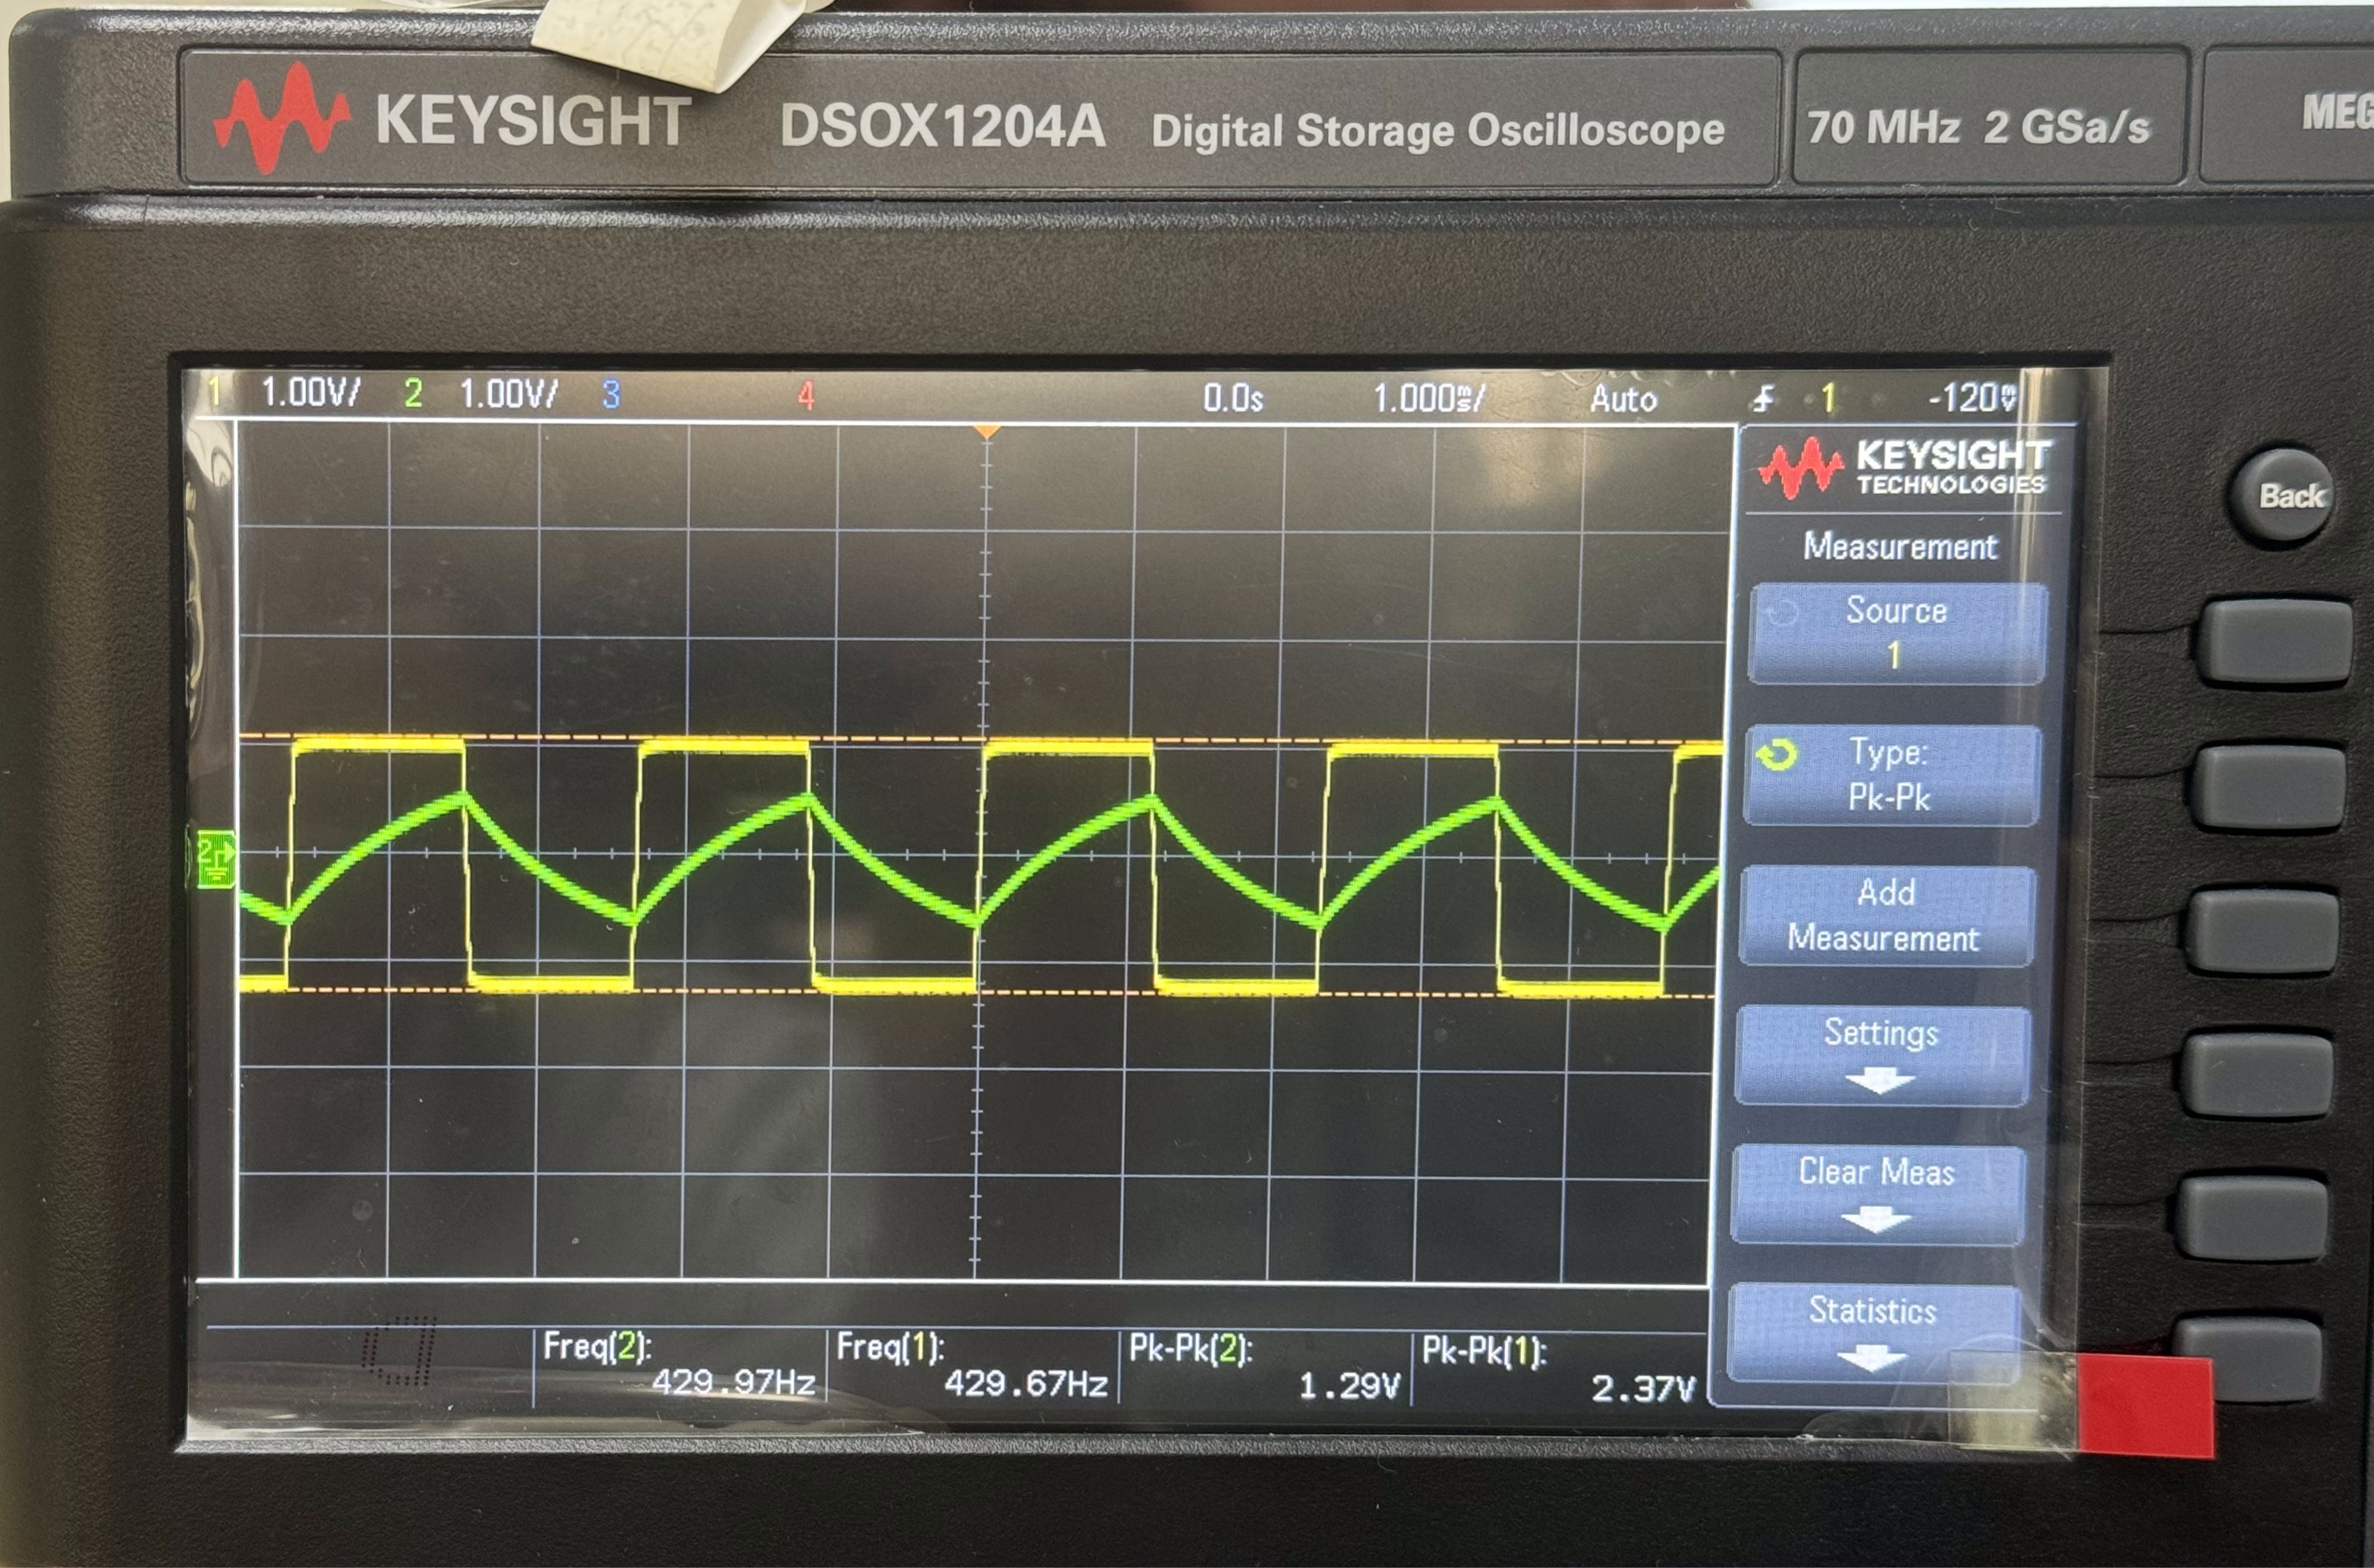
\includegraphics[width=0.7\linewidth]{Lab15/10k_10k.png}
        \caption{Observed Waveform of $R_4=R_5=10K\Omega$}
        \label{L510k10k}
    \end{figure}
    \FloatBarrier
    \begin{figure}[h]
        \centering
        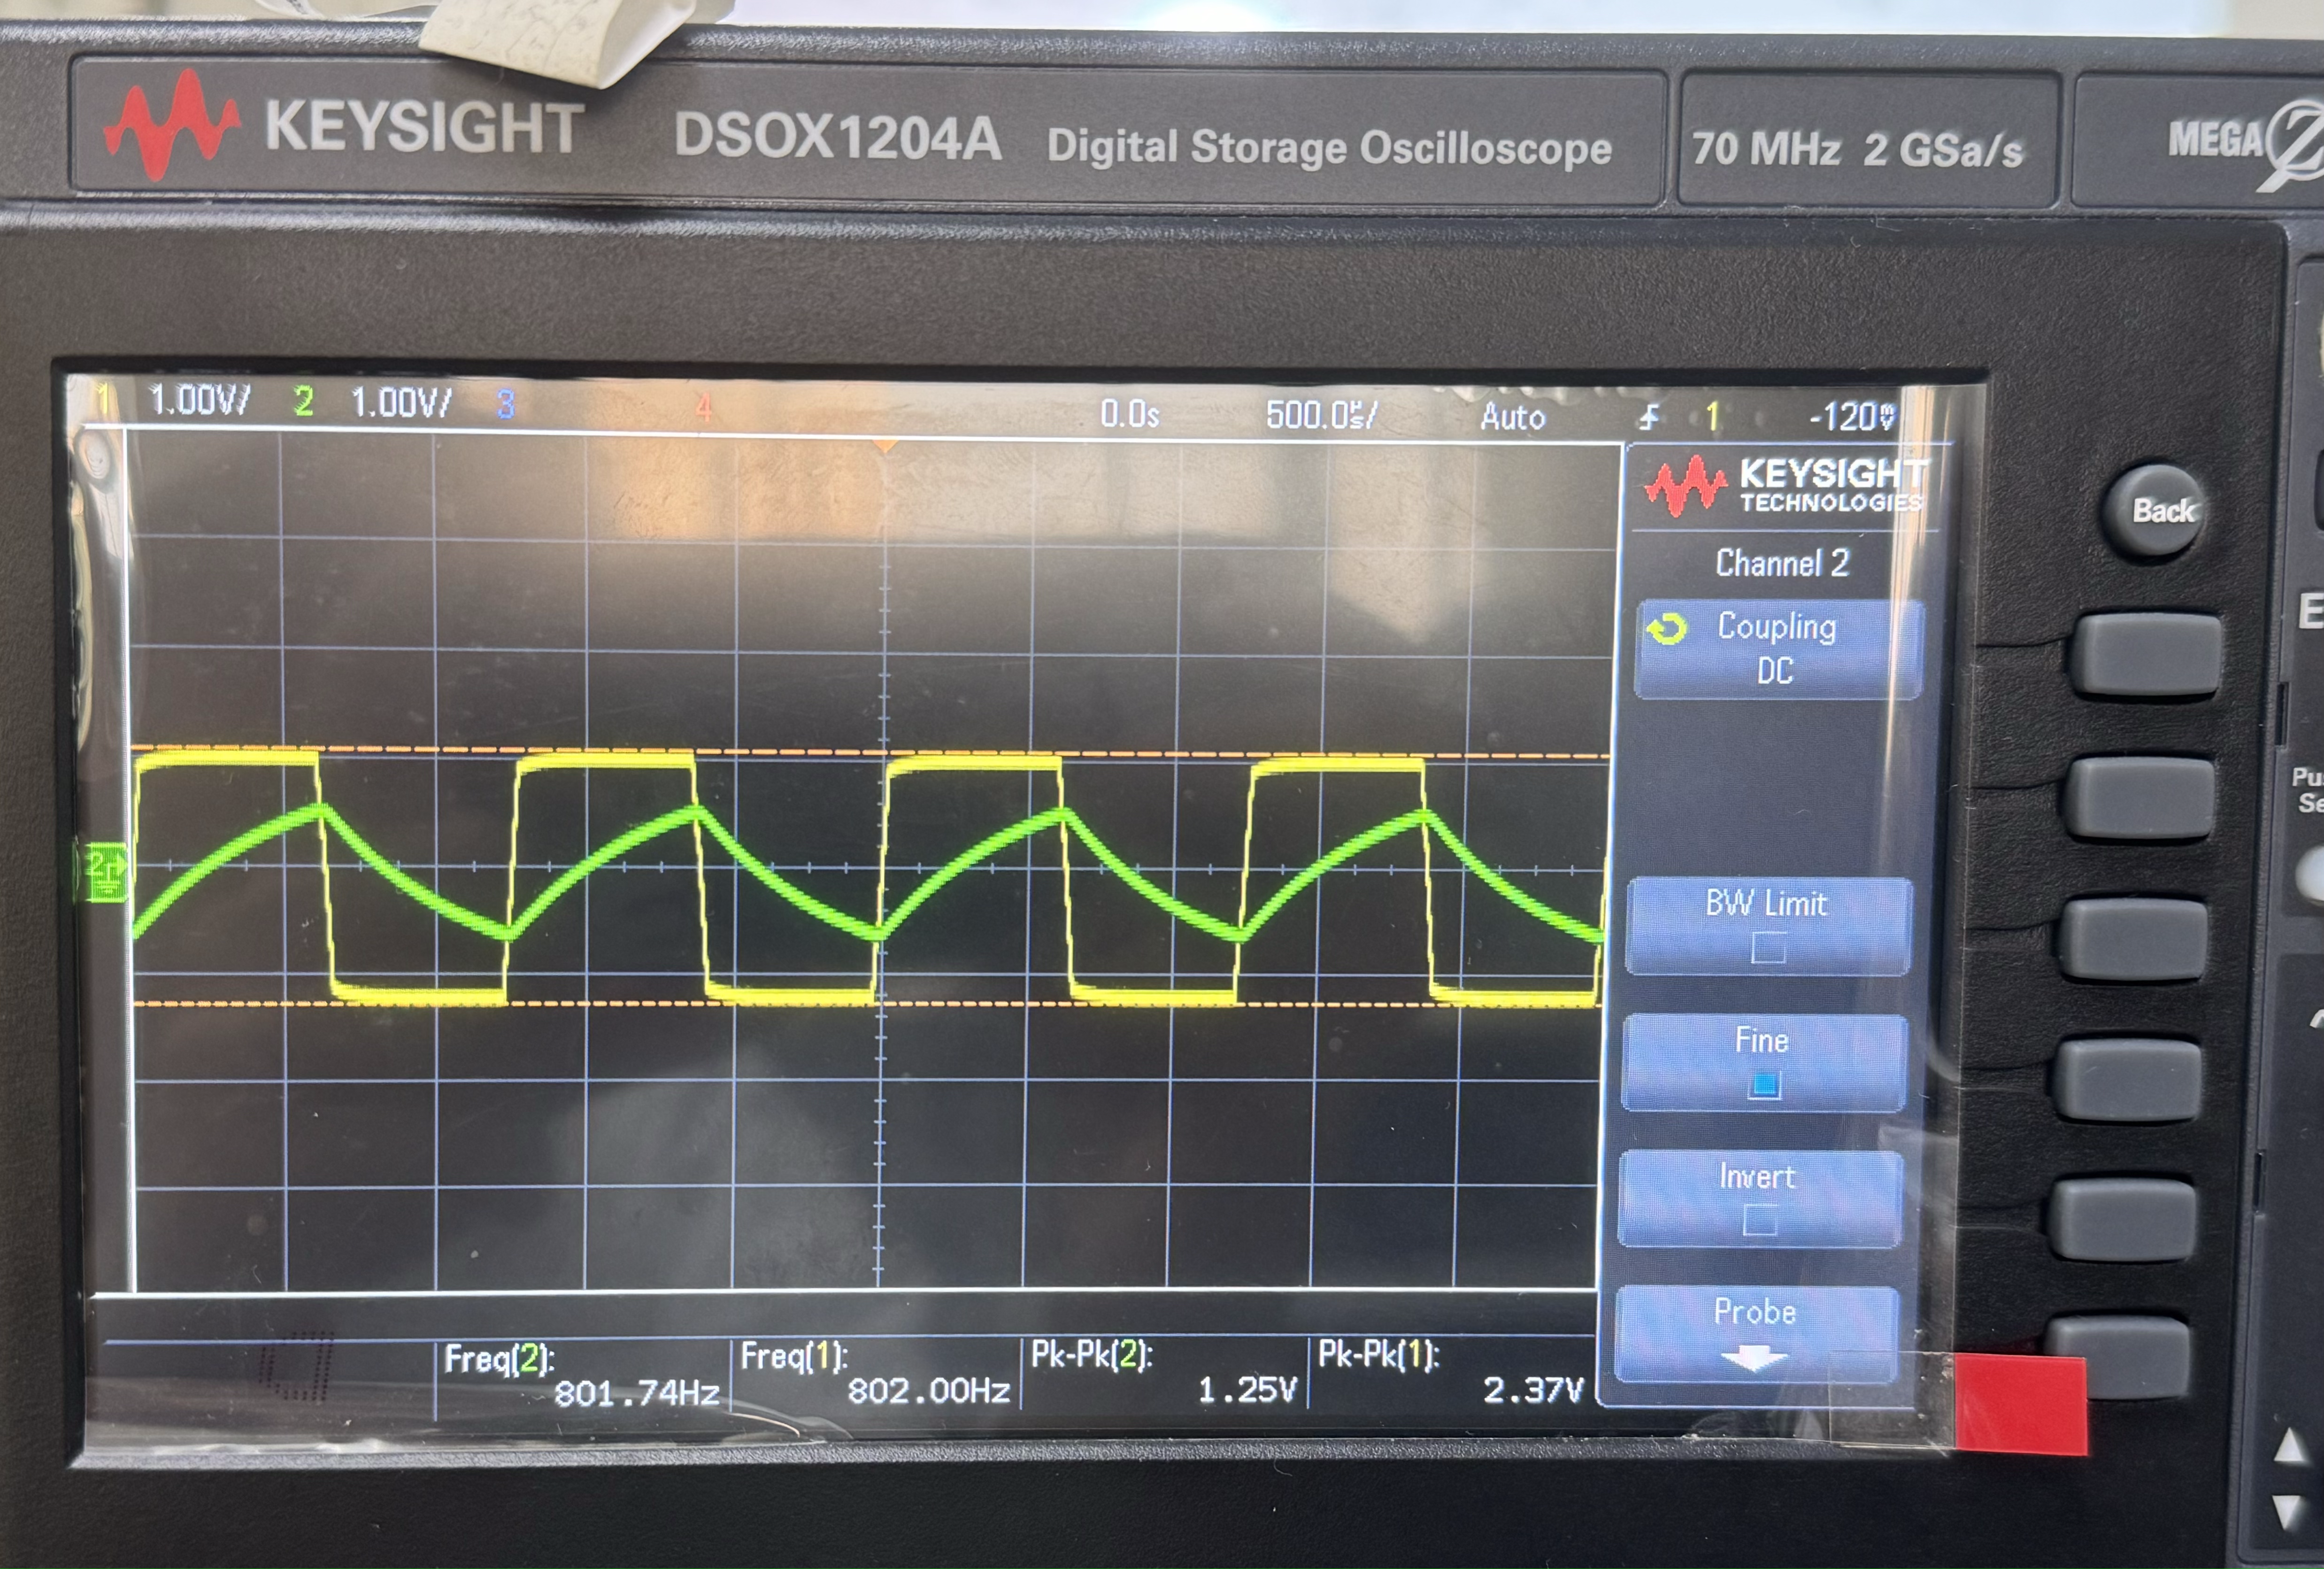
\includegraphics[width=0.7\linewidth]{Lab15/5k5k.png}
        \caption{Observed Waveform of $R_4=R_5=5K\Omega$}
        \label{L55k5k}
    \end{figure}
    \FloatBarrier
    \begin{figure}[h]
        \centering
        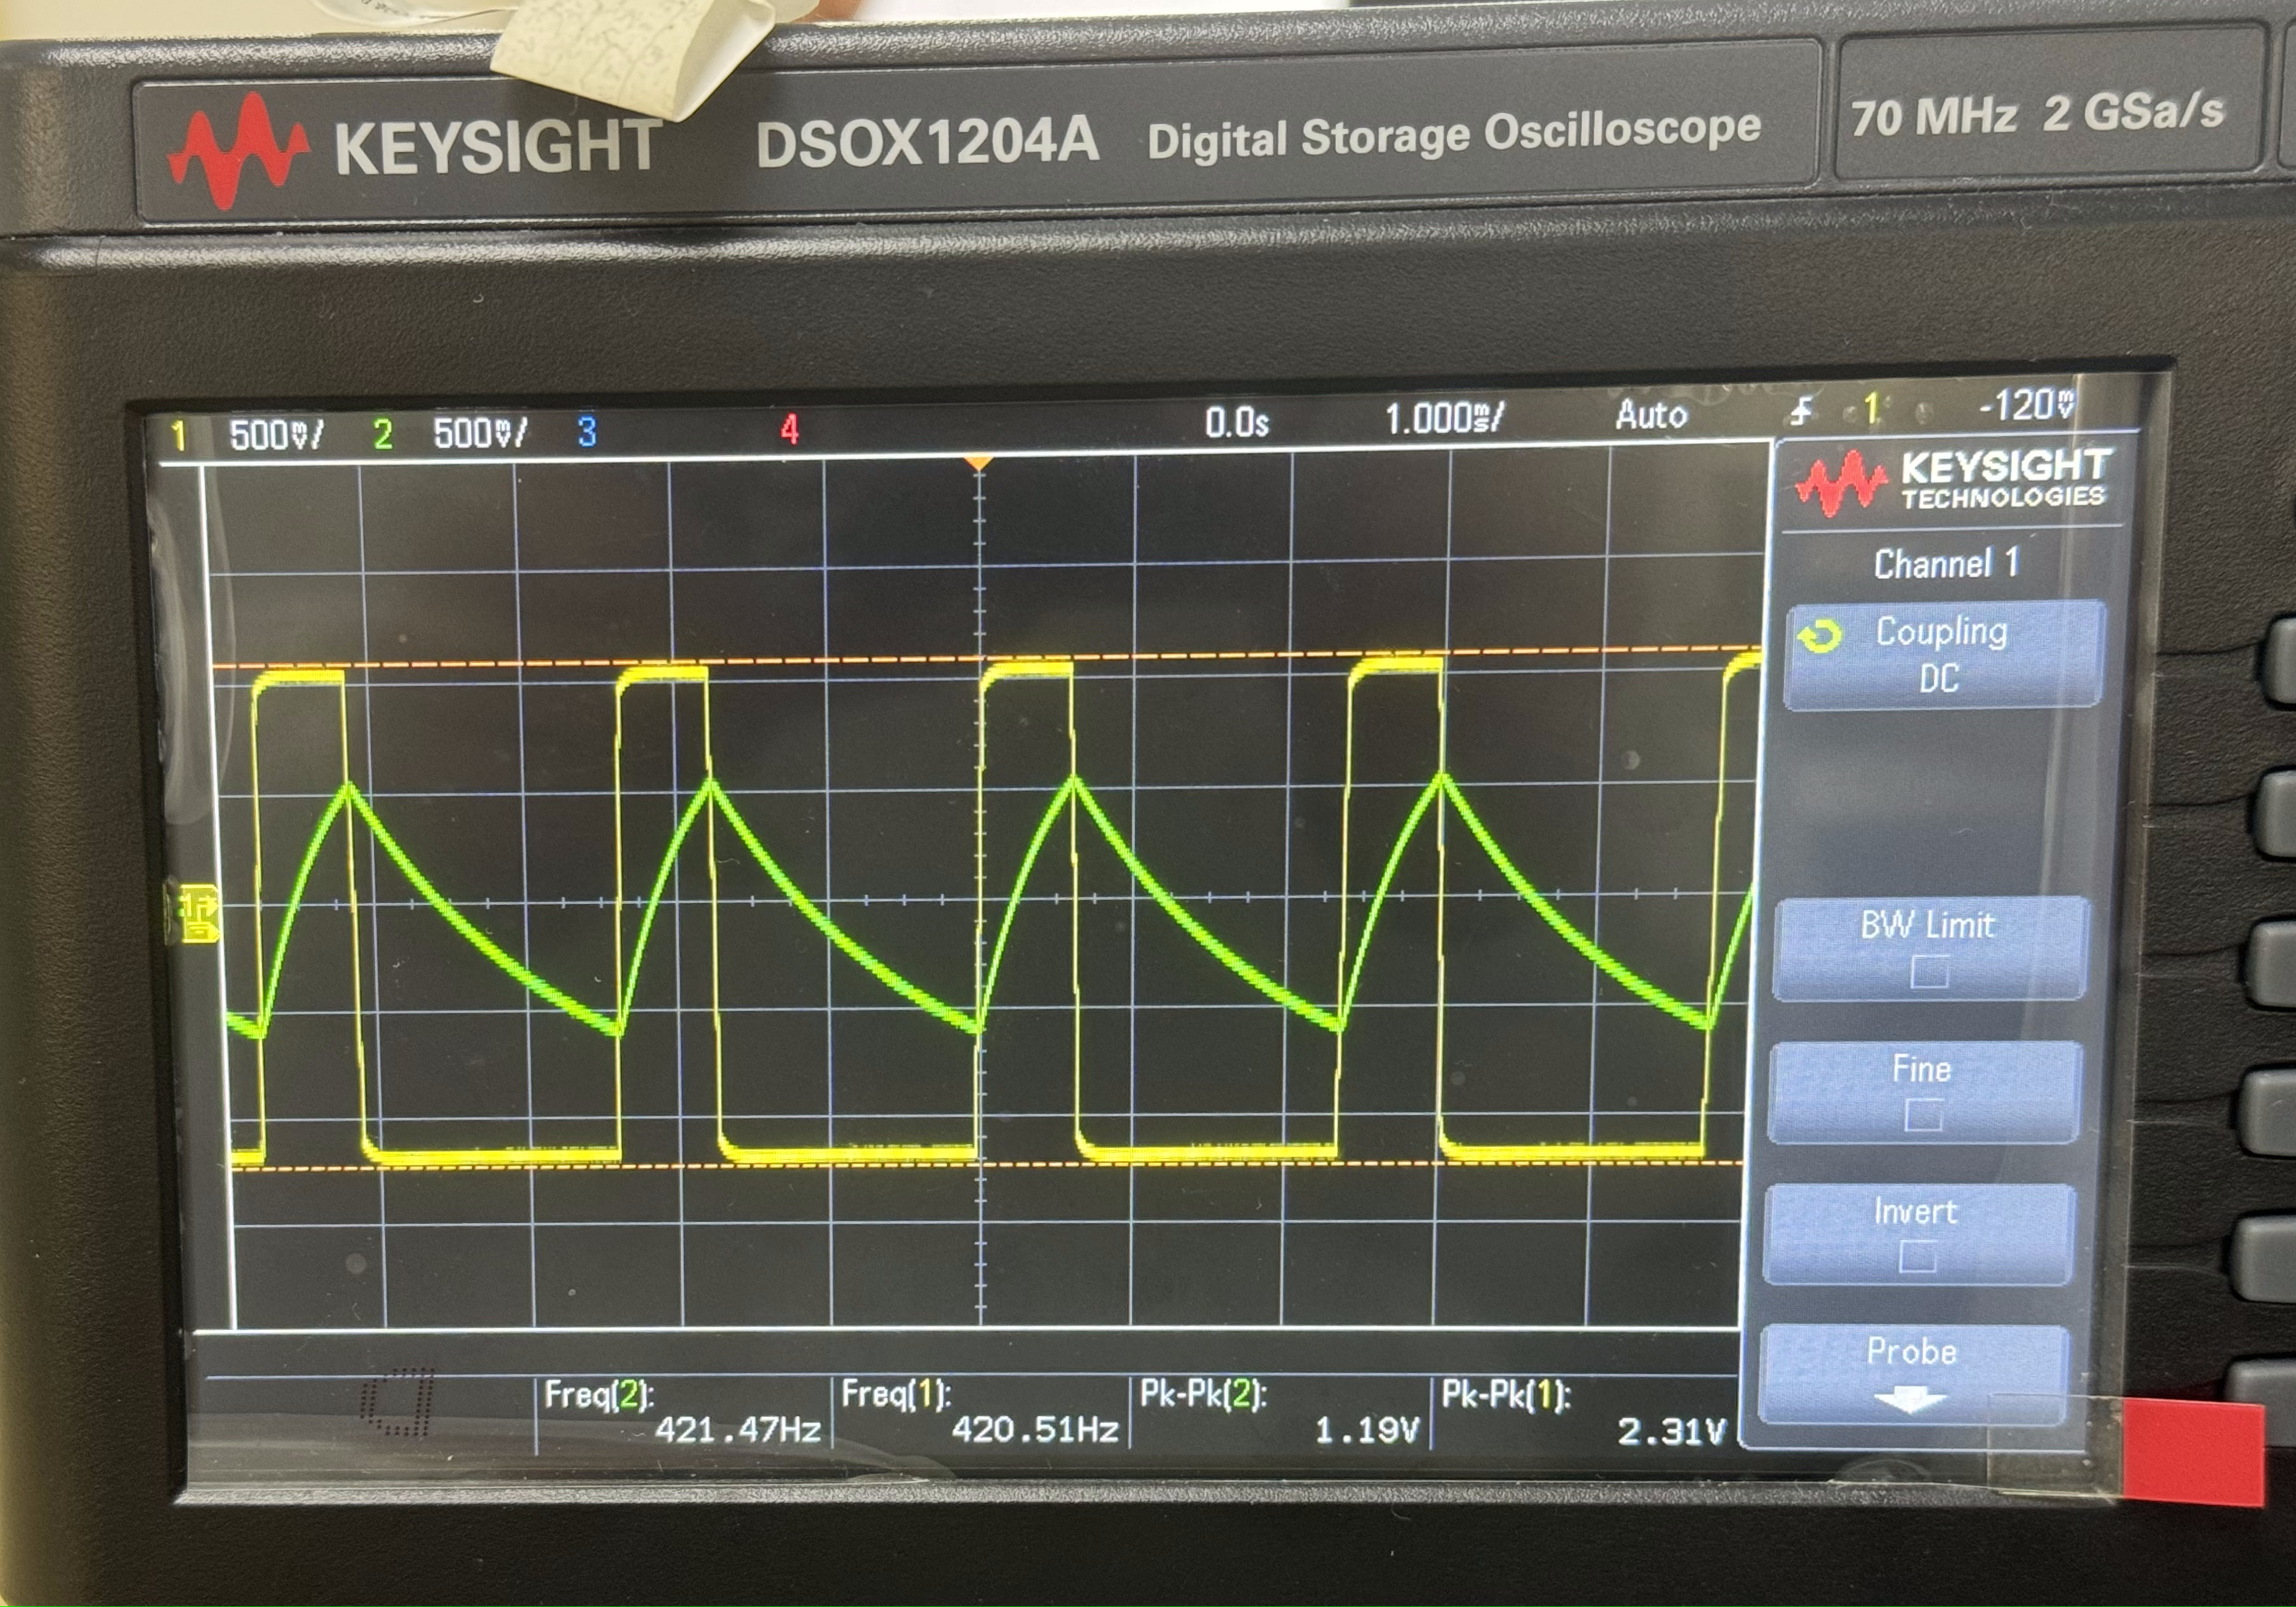
\includegraphics[width=0.7\linewidth]{Lab15/5k15k.png}
        \caption{Observed Waveform of $R_4=5k\Omega,~R_5=15K\Omega$}
        \label{L55k15k}
    \end{figure}
    \FloatBarrier
    The time required for the capacitor to charge and discharge is influenced by the resistors $R_4$ and $R_5$, respectively.\par
    An increase in the resistance of the resistor governing the capacitor's behavior results in a longer period for the capacitor's voltage to change.\par
    Conversely, a decrease in resistance reduces this period, as evidenced by the increase in the measured frequency ($f \propto \frac{1}{T}$) observed on the oscilloscope screen, as illustrated in Figure \ref{L510k10k} and Figure \ref{L55k5k}.
    Therefore, when the resistance of two resistors ($R_4$ \& $R_5$) is different, it will result in an asymmetry duration of high signal and low signal states.
    
\section{Discussion}
    Theoretically, configuring and enabling a wave generator requires a start-source to provide the initial power necessary to initiate signal oscillation within the circuit.\par
    However, in this experiment, the circuit was successfully built and operated without the use of a dedicated start-source to initiate the square-wave generator. This phenomenon can be attributed to minor static electricity present in the environment, which acted as a start-source to activate the circuit.

\section{Conclusion}
    In this experiment, we learned the fundamental principle of a wave generator constructed based on the operational amplifier. Furthermore, we gained more understanding of the impact of resistor on the capacitor within a small-signal RC circuit.\par
    Basically, the signal oscillation in the circuit is primarily facilitated by the capacitors, diode, and operational amplifier. The diode restricts the current flow to a specific direction, the capacitors store and release charge to stabilize the voltage signal over time, and the operational amplifier enhances the voltage signal to maintain oscillation.\par
    In detail, when the capacitor charges to a specific voltage threshold, $V_1$ exceeds $V_2$ (or vice versa), prompting the operational amplifier to output an inverted signal. In this scenario, $D_1$ turns off, $D_2$ turns on, and the signal reflects to the opposite direction along the y-axis.